\PassOptionsToPackage{unicode=true}{hyperref} % options for packages loaded elsewhere
\PassOptionsToPackage{hyphens}{url}
%
\documentclass[
]{article}
\usepackage{lmodern}
\usepackage{amssymb,amsmath}
\usepackage{ifxetex,ifluatex}
\ifnum 0\ifxetex 1\fi\ifluatex 1\fi=0 % if pdftex
  \usepackage[T1]{fontenc}
  \usepackage[utf8]{inputenc}
  \usepackage{textcomp} % provides euro and other symbols
\else % if luatex or xelatex
  \usepackage{unicode-math}
  \defaultfontfeatures{Scale=MatchLowercase}
  \defaultfontfeatures[\rmfamily]{Ligatures=TeX,Scale=1}
\fi
% use upquote if available, for straight quotes in verbatim environments
\IfFileExists{upquote.sty}{\usepackage{upquote}}{}
\IfFileExists{microtype.sty}{% use microtype if available
  \usepackage[]{microtype}
  \UseMicrotypeSet[protrusion]{basicmath} % disable protrusion for tt fonts
}{}
\makeatletter
\@ifundefined{KOMAClassName}{% if non-KOMA class
  \IfFileExists{parskip.sty}{%
    \usepackage{parskip}
  }{% else
    \setlength{\parindent}{0pt}
    \setlength{\parskip}{6pt plus 2pt minus 1pt}}
}{% if KOMA class
  \KOMAoptions{parskip=half}}
\makeatother
\usepackage{xcolor}
\IfFileExists{xurl.sty}{\usepackage{xurl}}{} % add URL line breaks if available
\IfFileExists{bookmark.sty}{\usepackage{bookmark}}{\usepackage{hyperref}}
\hypersetup{
  pdftitle={The statistical analysis of non-linear longitudinal data in biomedical research using generalized additive models},
  pdfauthor={Ariel Mundo; Timothy J. Muldoon; John R. Tipton},
  pdfborder={0 0 0},
  breaklinks=true}
\urlstyle{same}  % don't use monospace font for urls
\usepackage[margin=1in]{geometry}
\usepackage{longtable,booktabs}
% Allow footnotes in longtable head/foot
\IfFileExists{footnotehyper.sty}{\usepackage{footnotehyper}}{\usepackage{footnote}}
\makesavenoteenv{longtable}
\usepackage{graphicx,grffile}
\makeatletter
\def\maxwidth{\ifdim\Gin@nat@width>\linewidth\linewidth\else\Gin@nat@width\fi}
\def\maxheight{\ifdim\Gin@nat@height>\textheight\textheight\else\Gin@nat@height\fi}
\makeatother
% Scale images if necessary, so that they will not overflow the page
% margins by default, and it is still possible to overwrite the defaults
% using explicit options in \includegraphics[width, height, ...]{}
\setkeys{Gin}{width=\maxwidth,height=\maxheight,keepaspectratio}
\setlength{\emergencystretch}{3em}  % prevent overfull lines
\providecommand{\tightlist}{%
  \setlength{\itemsep}{0pt}\setlength{\parskip}{0pt}}
\setcounter{secnumdepth}{5}
% Redefines (sub)paragraphs to behave more like sections
\ifx\paragraph\undefined\else
  \let\oldparagraph\paragraph
  \renewcommand{\paragraph}[1]{\oldparagraph{#1}\mbox{}}
\fi
\ifx\subparagraph\undefined\else
  \let\oldsubparagraph\subparagraph
  \renewcommand{\subparagraph}[1]{\oldsubparagraph{#1}\mbox{}}
\fi

% set default figure placement to htbp
\makeatletter
\def\fps@figure{htbp}
\makeatother

\usepackage{subfig}
\usepackage{breqn}
\usepackage[font={small}]{caption}
\usepackage{float}

\title{\textbf{The statistical analysis of non-linear longitudinal data in biomedical research using generalized additive models}}
\usepackage{etoolbox}
\makeatletter
\providecommand{\subtitle}[1]{% add subtitle to \maketitle
  \apptocmd{\@title}{\par {\large #1 \par}}{}{}
}
\makeatother
\subtitle{\emph{Beyond repeated measures ANOVA and Linear Mixed Models}}
\author{Ariel Mundo\footnote{Department of Biomedical Engineering, University of Arkansas, Fayetteville} \and Timothy J. Muldoon\footnote{Department of Biomedical Engineering, University of Arkansas, Fayetteville} \and John R. Tipton\footnote{Department of Mathematical Sciences, University of Arkansas, Fayetteville}}
\date{}

\begin{document}
\maketitle

{
\setcounter{tocdepth}{2}
\tableofcontents
}
\hypertarget{background}{%
\section{Background}\label{background}}

Longitudinal studies are designed to repeatedly measure a variable of interest in a group (or groups) of subjects, with the intention of observing the evolution of effect across time rather than analyzing a single time point (e.g., a cross-sectional study). Biomedical research frequently uses longitudinal studies to analyze the evolution of a ``treatment'' effect across multiple time points; and in such studies the subjects of analysis range from animals (mice, rats, rabbits), to human patients, cells, or blood samples, among many others. Tumor response {[}1--4{]}, antibody expression {[}5,6{]}, and cell metabolism {[}7,8{]} are examples of the different situations where researchers have used longitudinal designs to study some physiological response. Because the frequency of the measurements in a longitudinal study is dependent on the biological phenomena of interest and the experimental design of the study, the frequency of such measurements can range from minute intervals to study a short-term response such as anesthesia effects in animals{[}9{]}, to weekly measurements to analyze a mid-term response like the evolution of dermatitis symptoms in breast cancer patients {[}10{]}, to monthly measurements to study a long-term response such as mouth opening following RT in neck cancer patients {[}11{]}.

Traditionally, a ``frequentist'' or ``classical'' statistical paradigm is used in biomedical research to derive inferences from a longitudinal study. The frequentist paradigm regards probability as a limiting frequency {[}12{]} by assuming a null hypothesis under a statistical model that is often an \emph{analysis of variance over repeated measures} (repeated measures ANOVA or rm-ANOVA). The rm-ANOVA model makes three key assumptions regarding longitudinal data: 1) linearity of the response across time, 2) constant correlation across same-subject measurements, and 3) observations from each subject are obtained at all time points through the study (a condition also known as \emph{complete observations}) {[}13,14{]}.

The expected linear behavior of the response through time is a key requisite in rm-ANOVA {[}15{]}. This ``linearity assumption'' in rm-ANOVA implies that the model is misspecified when the data does not follow a linear trend, which results in unreliable inference. In biomedical research, non-linear trends are the norm rather than the exception in longitudinal studies. A particular example of this non-linear behavior in longitudinal data arises in measurements of tumor response in preclinical and clinical settings {[}1,8,16{]}. These studies have shown that the collected signal does not follow a linear trend over time, and presents extreme variability at different time points, making the fit of rm-ANOVA model inconsistent with the observed variation. Therefore, when rm-ANOVA is used to draw inference of such highly-variable data the estimates are inevitably biased, because the model is only able to accommodate linear trends that are far from adequately representing the biological phenomenon of interest.

A \emph{post hoc} analysis is the statistical test used in conjunction with rm-ANOVA to perform repeated comparisons to estimate a \emph{p-value}, which in turn is used as a measure of significance.
Although it is possible that a \emph{post hoc} analysis of rm-ANOVA is able to find ``significant'' \emph{p-values}( \emph{p}\textless{}0.05) from non-linear data, the validity of such metric is dependent on how adequate the model fits the data. In other words, \emph{p-values} are valid only if the model and the data have good agreement; if that is not the case, a ``Type III'' error (known as ``model misspecification'') occurs{[}17{]}. For example, model misspecification will occur when a model that is only able to explain linear responses (such as rm-ANOVA) is fitted to data that follows a quadratic trend, thereby causing the resulting \emph{p-values} and parameter estimates to be invalid {[}18{]}.

Additionally, the \emph{p-value} itself is highly variable, and multiple comparisons can inflate the false positivity rate (Type I error or \(\alpha\)) {[}19,20{]}, consequently biasing the conclusions of the study. Corrections exist to address the Type I error issue of multiple comparisons (such as Bonferroni {[}21{]}), but they in turn reduce statistical power (1-\(\beta\)){[}22{]}, and lead to increased Type II error (failing to reject the null hypothesis when the null hypothesis is false) {[}23,24{]}. Therefore, the tradeoff of \emph{post hoc} comparisons in rm-ANOVA between Type I, II and III errors might be difficult to balance in a biomedical longitudinal study where a delicate balance exists between statistical power and sample size.

On the other hand, the assumption of constant correlation in rm-ANOVA (often known as the \emph{compound symmetry assumption}) is typically unreasonable because correlation between the measured responses often diminishes as the time interval between the observation increases {[}25{]}. Corrections can be made in rm-ANOVA in the absence of compound symmetry {[}26,27{]}, but the effectiveness the correction is limited by the size of the sample, the number of measurements{[}28{]}, and group sizes {[}29{]}. In the case of biomedical research, where living subjects are frequently used, sample sizes are often not ``large'' due to ethical and budgetary reasons {[}30{]} which might cause the corrections for lack of compound symmetry to be ineffective.

Due to a variety of causes, the number of observations during a study can vary between all subjects. For example, in a clinical trial patients may voluntarily withdraw, whereas attrition due to injury or weight loss in preclinical animal studies is possible. It is even plausible that unexpected complications with equipment or supplies arise that prevent the researcher from collecting measurements at certain time points. In each of these missing data scenarios,the \emph{complete observations} assumption of classical rm-ANOVA is violated. When incomplete observations occur, a rm-ANOVA model is fit by excluding all subjects with missing observations from the analysis {[}13{]}. This elimination of partially missing data from the analysis can result in increased costs if the desired statistical power is not met with the remaining observations, because it would be necessary to enroll more subjects. At the same time, if the excluded observations contain insightful information that is not used, their elimination from the analysis may limit the demonstration of significant differences between groups.

During the last decade, the biomedical community has started to recognize the limitations of rm-ANOVA in the analysis of longitudinal information. The recognition on the shortcomings of rm-ANOVA is exemplified by the use of linear mixed effects models (LMEMs) by certain groups to analyze longitudinal tumor response data {[}8,16{]}. Briefly, LMEMs incorporate \emph{fixed effects}, which correspond to the levels of experimental factors in the study (e.g., the different drug regimens in a clinical trial), and \emph{random effects}, which account for random variation within the population (e.g., the individual-level differences not due to treatment such as weight or age). When compared to the traditional rm-ANOVA, LMEMs are more flexible as they can accommodate missing observations for multiple subjects and allow different modeling strategies for the variability within each measure in every subject {[}15{]}. However, LMEMs impose restrictions in the distribution of the errors of the random effects, which need to be normally distributed and independent {[}13,31{]}. And even more importantly, LMEMs also expect a linear relationship between the response and time {[}15{]}, making them unsuitable to analyze non-linear data.

As the rm-ANOVA and the more flexible LMEM approaches make overly restrictive assumptions regarding the linearity of the response, there is a need for biomedical researchers to explore the use of additional statistical tools that allow the data (and not an assumption in trend) to determine the trend of the fitted model, to enable appropriate inference.

In this regard, generalized additive models (GAMs) present an alternative approach to analyze longitudinal data. Although not frequently used by the biomedical community, these non-parametric models are customarily used in other fields to analyze longitudinal data. Examples of the use of GAMs include the analysis of temporal variations in geochemical and palaeoecological data {[}32--34{]}, health-environment interactions {[}35{]} and the dynamics of government in political science {[}36{]} . There are several advantages of GAMs over LMEMs and rm-ANOVA models: 1) GAMs can fit a more flexible class of smooth responses that enable the data to dictate the trend in the fit of the model, 2) they can model non-constant correlation between repeated measurements {[}37{]} and 3) can easily accommodate missing observations. Therefore, GAMs can provide a more flexible statistical approach to analyze non-linear biomedical longitudinal data than LMEMs and rm-ANOVA.

The current advances in programming languages designed for statistical analysis (specifically \(\textsf{R}\)), have eased the computational implementation of traditional models such as rm-ANOVA and more complex approaches such as LMEMs and GAMs. In particular, \(\textsf{R}\){[}38{]} has an extensive collection of documentation and functions to fit GAMs in the package \emph{mgcv} {[}37,39{]} that not only speed up the initial stages of the analysis but also enable the use of advanced modeling structures (e.g.~hierarchical models, confidence interval comparisons) without requiring advanced programming skills from the user. At the same time, \(\textsf{R}\) has many tools that simplify data simulation, an emerging strategy used to test statistical models {[}28{]}. Data simulation methods allow the researcher to create and explore different alternatives for analysis without collecting information in the field, reducing the time window between experiment design and its implementation, and simulation can be also used for power calculations and study design questions.

This work provides biomedical researchers with a clear understanding of the theory and the practice of using GAMs to analyze longitudinal data using by focusing on four areas. First, the limitations of LMEMs and rm-ANOVA regarding linearity of response, constant correlation structures and missing observations is explained in detail. Second, the key theoretical elements of GAMs are presented using clear and simple mathematical notation while explaining the context and interpretation of the equations. Third, using simulated data that reproduces patterns in previously reported studies {[}16{]} we illustrate the type of non-linear longitudinal data that often occurs in biomedical research. The simulated data experiments highlight the differences in inference between rm-ANOVA, LMEMs and GAMs on data similar to what is commonly observed in biomedical studies. Finally, reproducibility is emphasized by providing the code to generate the simulated data and the implementation of different models in \(\textsf{R}\), in conjunction with a step-by-step guide demonstrating how to fit models of increasing complexity.

In summary, this work will allow biomedical researchers to identify when the use of GAMs instead of rm-ANOVA or LMEMs is appropriate to analyze longitudinal data, and provide guidance on the implementation of these models by improving the standards for reproducibility in biomedical research.

\hypertarget{challenges-presented-by-longitudinal-studies}{%
\section{Challenges presented by longitudinal studies}\label{challenges-presented-by-longitudinal-studies}}

\hypertarget{the-repeated-measures-anova}{%
\subsection{The repeated measures ANOVA}\label{the-repeated-measures-anova}}

The \emph{repeated measures analysis of variance} (rm-ANOVA) is the standard statistical analysis for longitudinal data in biomedical research. This statistical methodology requires certain assumptions for the model to be valid. From a practical view, the assumptions can be divided in three areas: 1) linear relationship between covariates and response, 2) a constant correlation between measurements, and, 3) complete observations for all subjects. Each one of these assumptions is discussed below.

\hypertarget{linear-relationship}{%
\subsection{Linear relationship}\label{linear-relationship}}

\hypertarget{the-repeated-measures-anova-case}{%
\subsubsection{The repeated measures ANOVA case}\label{the-repeated-measures-anova-case}}

In a biomedical longitudinal study, two or more groups of subjects (e.g., patients, mice, samples) are subject to different treatments (e.g., a ``treatment'' group receives a novel drug vs.~a ``control'' group that receives a placebo), and measurements from each subject within each group are collected at specific time points. The collected response is modeled with \emph{fixed} components. The \emph{fixed} component can be understood as a constant value in the response which the researcher is interested in measuring, i.e., the average effect of the novel drug in the ``treatment'' group.

Mathematically speaking, a rm-ANOVA model with an interaction can be written as:

\begin{equation}
y_{ijt} = \beta_0+ \beta_1 \times time_{t} + \beta_2 \times treatment_{j} + \beta_3 \times time_{t}\times treatment_{j}+\varepsilon_{tij}\\ 
\label{eq:linear-model}
\end{equation}

In this model \(y_{ijt}\) is the response for subject \(i\), in treatment group \(j\) at time \(t\), which can be decomposed in a mean value \(\beta_0\), \emph{fixed effects} of time (\(time_t\)), treatment (\(treatment_j\)) and their interaction \(time_t*treatment_j\) which have linear slopes given by \(\beta_1, \beta_2\) and \(\beta_3\), respectively. Independent errors \(\varepsilon_{tij}\) represent random variation not explained by the \emph{fixed} effects, and are assumed to be \(\sim N(0,\sigma^2)\).
In a biomedical research context, suppose two treatments groups are used in a study (e.g., ``placebo'' vs.~``novel drug'' or ``saline'' vs.~``chemotherapy''). Then, the group terms in Equation \eqref{eq:linear-model} can be written as below with \(treatment_j=0\) representing the first treatment group (Group A) and \(treatment_j=1\) representing the second treatment group (Group B). The linear models then can be expressed as

\begin{equation}
y_{ijt} = \begin{cases}
\beta_0 + \beta_1\times time_{t}+\mu_{ijt}+\varepsilon_{ijt}   & \mbox{if Group A}\\
\beta_0 + \beta_1 \times time_{t} + \beta_2 \times +\beta_3 \times time_{t} \times +\mu_{ijt}+\varepsilon_{ijt}  & \mbox{if Group B}\\
\end{cases}
\label{eq:ANOVA-by-group}
\end{equation}

To further simplify the expression, substitute \(\widetilde{\mu}=\beta_0+\beta_{2}\) and \(\widetilde{\beta_{1}}=\beta_{1}+\beta_{3}\) in the equation for Group B. This substitution allows for a different intercept and slope for Groups A and B. The model is then written as

\begin{equation}
y_{ijt} = \begin{cases}
\beta_0 + \beta_1\times time_{t}+\mu_{ijt}+\varepsilon_{ijt}   & \mbox{if Group A}\\
\widetilde{\mu} + \widetilde{\beta_1} \times time_{t} +\mu_{ijt}+\varepsilon_{ijt}  & \mbox{if Group B}\\
\end{cases}
\label{eq:ANOVA-lines}
\end{equation}

Presenting the model in this manner makes clear that when treating different groups, an rm-ANOVA model is able to accommodate non-parallel lines in each case (different intercepts and slopes per group). In other words, the rm-ANOVA model ``expects'' a linear relationship between the covariates and the response, this means that either presented as Equation \eqref{eq:linear-model}, Equation \eqref{eq:ANOVA-by-group} or Equation \eqref{eq:ANOVA-lines}, an rm-ANOVA model is only able to accommodate linear patterns in the data. If the data show non-linear behavior, the rm-ANOVA model will approximate this behavior with non-parallel lines.

\hypertarget{the-linear-mixed-model-case}{%
\subsubsection{The Linear Mixed Model Case}\label{the-linear-mixed-model-case}}

A linear mixed model (LMEM) is a class of statistical model that incorporates \emph{fixed effects} to model the relationship between the covariates and the response, and \emph{random effects} to model subject variability that is not the primary focus of the study but that might be important to distinguish {[}15,40{]}. A LMEM with interaction between time and treatment for a longitudinal study can be written as:

\begin{equation}
y_{ijt} = \beta_0+ \beta_1 \times time_{t} + \beta_2 \times treatment_{j} + \beta_3 \times time_{t}\times treatment_{j}+\mu_{ij} +\varepsilon_{tij}\\ 
\label{eq:LMEM}
\end{equation}

When Equation \eqref{eq:linear-model} and Equation \eqref{eq:LMEM} are compared, it is easily noticeable that LMEM and rm-ANOVA have the same construction regarding the \emph{fixed effects} of time and treatment, but that the LMEM incorporates an additional source of variation (the term \(\mu_{ij}\)). This term \(\mu_{ij}\) is the one that corresponds to the \emph{random effect}, accounting for variability in each subject within each group. The \emph{random} component can also be understood as used to model some ``noise'' in the response, but that is intended to be analyzed and disentangled from the ``global noise'' term \(\varepsilon_{tij}\) from Equation \eqref{eq:linear-model}.

For example, if the blood concentration of the drug is measured in certain subjects in the early hours of the morning while other subjects are measured in the afternoon, it is possible that the difference in the collection time introduces some ``noise'' in the data. As the name suggests, this ``random'' variability needs to be modeled as a variable rather than as a constant value. The \emph{random effect} \(\mu_{ij}\) in Equation \eqref{eq:LMEM} is assumed to be independently normally distributed with mean zero and variance \(\sigma^2_\mu\), which can be expressed as \(\mu_{ij} \sim N(0,\sigma^2_\mu)\). In essence,the \emph{random effect} in a LMEM enables to fit models with different slopes at the subject-level{[}15{]}. However,the expected linear relationship of the covariates and the response in Equation \eqref{eq:linear-model} and in Equation \eqref{eq:LMEM} is essentially the same, representing a major limitation of LMEMs to fit a non-linear response.

\hypertarget{covariance-in-rm-anova-and-lmems}{%
\subsection{Covariance in rm-ANOVA and LMEMs}\label{covariance-in-rm-anova-and-lmems}}

In a longitudinal study there is an expected \emph{covariance} between repeated measurements on the same subject, and because repeated measures occur in the subjects within each group, there is a \emph{covariance} between measurements at each time point within each group. The \emph{covariance matrix} (also known as the variance-covariance matrix) is a matrix that captures the variation between and within subjects in a longitudinal study{[}41{]} (For an in-depth analysis of the covariance matrix see {[}40,42{]}).

In the case of an rm-ANOVA analysis, it is typically assumed that the covariance matrix has a specific construction known as \emph{compound symmetry} (also known as ``sphericity'' or ``circularity''). Under this assumption, the between-subject variance and within-subject correlation are constant across time {[}26,42,43{]}. However, it has been shown that this condition is frequently not justified because the correlation between measurements tends to change over time {[}44{]}; and it is higher between consecutive measurements {[}13,25{]}. Although corrections can be made (such as Huyhn-Feldt or Greenhouse-Geisser){[}26,27{]} the effectiveness of each correction is limited because it depends on the size of the sample,the number of repeated measurements{[}28{]}, and they are not robust if the group sizes are unbalanced {[}29{]}. Because biomedical longitudinal studies are often limited in sample size and can have an imbalanced design, the corrections required to use an rm-ANOVA model may not be able to provide a reasonable adjustment that makes the model valid.

In the case of LMEMs, one key advantage over rm-ANOVA is that they allow different structures for the variance-covariance matrix including exponential, autoregressive of order 1, rational quadratic and others {[}15{]}. Nevertheless, the analysis required to determine an appropriate variance-covariance structure for the data can be a long process by itself. Overall, the spherical assumption for rm-ANOVA may not capture the natural variations of the correlation in the data, and can bias the inferences from the analysis.

\hypertarget{missing-observations}{%
\subsection{Missing observations}\label{missing-observations}}

Missing observations are an issue that arises frequently in longitudinal studies. In biomedical research, this situation can be caused by reasons beyond the control of the investigator {[}45{]}. Dropout from patients and attrition or injury in animals are among the reasons for missing observations. Statistically, missing information can be classified as \emph{missing at random} (MAR), \emph{missing completely at random} (MCAR), and \emph{missing not at random} (MNAR) {[}42{]}. In a MAR scenario, the pattern of the missing information is related to some variable in the data, but it is not related to the variable of interest {[}46{]}. If the data are MCAR, this means that the missingness is completely unrelated to the collected information {[}47{]}, and in the case of MNAR the missing values are dependent on their value. An rm-ANOVA model assumes complete observations for all subjects, and therefore subjects with one or more missing observations are excluded from the analysis. This is inconvenient because the remaining subjects might not accurately represent the population, and statistical power is affected by this reduction in sample size {[}48{]}.

In the case of LMEMs, inferences from the model are valid when missing observations in the data exist that are MAR or MCAR {[}40{]}. For example, if attrition occurs in all mice that had lower weights at the beginning of a chemotherapy response study, the missing data can be considered MAR because the missigness is unrelated to other variables of interest.

This section has presented the assumptions for analyzing longitudinal data using rm-ANOVA and LMEMs and compared their differences regarding linearity, the covariance matrix and missing data. Of notice, LMEMs offer a more robust and flexible approach than rm-ANOVA and if the data follows a linear trend, they provide an excellent choice to derive inferences from a repeated measures study. However, when the data presents high a non-linear behavior, LMEMs and rm-ANOVA fail to capture the trend of the data. To better convey the issues of linearity and correlation in linear models fitted to non-linear data, simulation is used in the next section.

\hypertarget{simulation}{%
\subsection{How does an rm-ANOVA fit looks like? A visual representation using simulation}\label{simulation}}

To demonstrate the limitations of rm-ANOVA an LMEMs for non-linear longitudinal data, this section presents a simulation experiment of a normally distributed response of two groups of 10 subjects each. An rm-ANOVA model (Equation \eqref{eq:linear-model}) is fitted to each group, using \(\textsf{R}\){[}38{]} and the package \emph{nlme}{[}49{]}.
Briefly, two cases for the mean responses for each group are considered: in the first case, the mean response in each group is a linear function with different intercepts and slopes; a negative slope is used for Group 1 and a positive slope is used for Group 2 (Figure @ref(fig:l-q-response, A)). In the second case, a second-degree polynomial (quadratic) function is used for the mean response per group: the quadratic function is concave down for Group 1 and it is concave up for Group 2 (Figure \ref{fig:l-q-response}, C). In both the linear and quadratic simulated data, the groups start with the same mean value at the first time point. This is intentional in order to simulate the expected temporal evolution of some physiological quantity.

Specifically, the rationale for the chosen linear and quadratic functions is the likelihood that a measured response in two treatment groups is similar in the initial phase of the study, but as treatment progresses a divergence in the trend of the response indicates a difference in the effect of each treatment. In other words, Group 1 can be thought as a ``Control'' group and Group 2 as a ``Treatment'' group. From the mean response per group (linear or quadratic), the variability or ``error'' of individual responses within each group is simulated using a covariance matrix with compound symmetry (constant variance across time). Thus, the response per subject in both the linear and quadratic simulation corresponds to the mean response per group plus the error (Figure \ref{fig:l-q-response} B,D). A more comprehensive exploration of the fit of rm-ANOVA for linear and non-linear longitudinal data is in Figure \ref{fig:linear-cases} and Figure \ref{fig:quadratic-cases} in the Appendix, where simulation with compound symmetry and independent errors (errors generated from a a normal distribution that are not constant over time) and the plot of simulated errors, and fitted parameters in presented.

\begin{figure}[!h]

{\centering 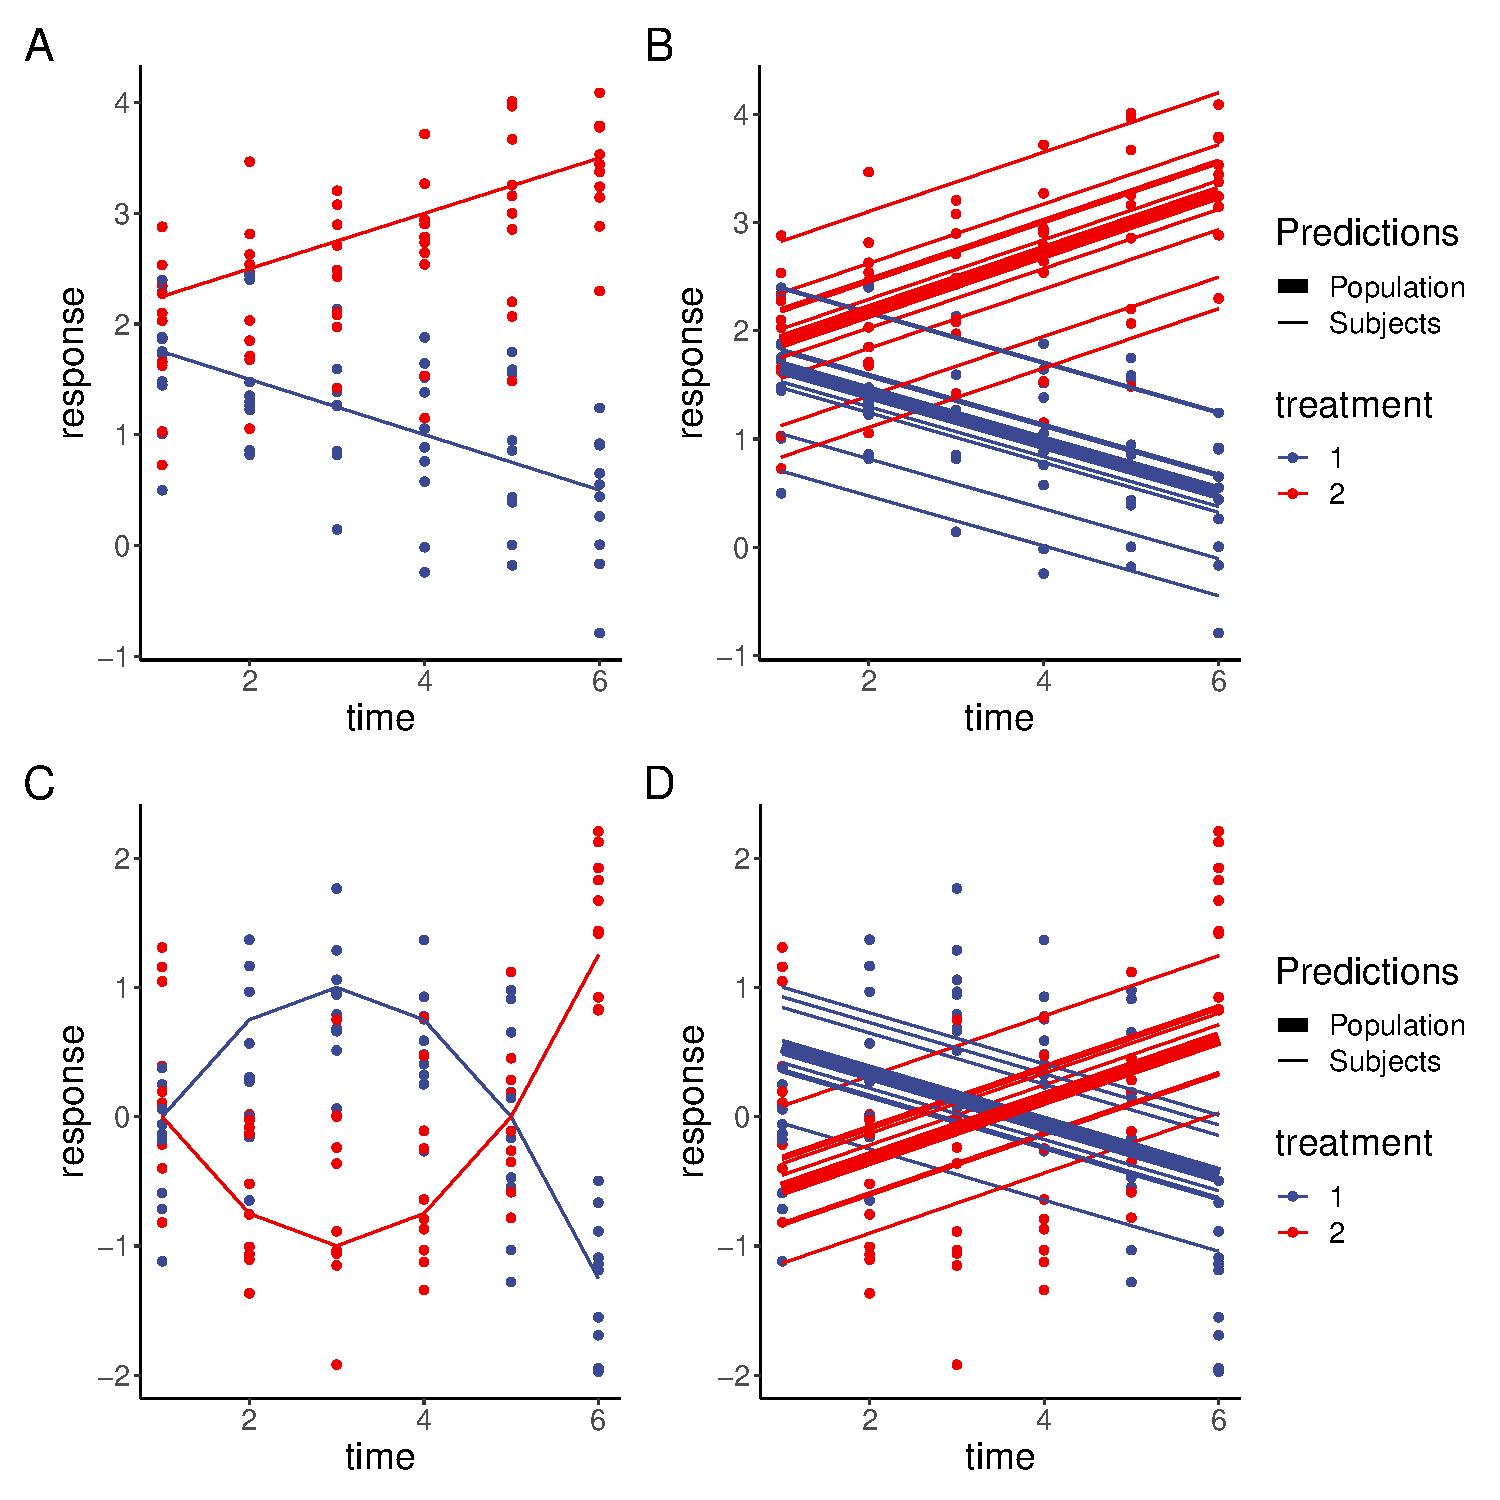
\includegraphics[width=0.75\linewidth,]{Manuscript_AM_v4_files/figure-latex/l-q-response-1} 

}

\caption{Simulated linear responses from two groups with correlated (top row) or independent (bottom row) errors using a rm-ANOVA model. A, C:Simulated data with known mean response (linear or quadratic, thin lines) and individual responses (points) showing the dispersion of the data. B,D: Estimations from the rm-ANOVA model for the mean group response (linear of quadratic). Thick lines are the predicted mean response per group, thin lines are the random effects for each subject and points represent the original raw data. The rm-ANOVA model does not pick the trend of the quadratic data.}\label{fig:l-q-response}
\end{figure}

The simulation shows that the fit produced by the rm-ANOVA model is good for linear data, as the predictions for the mean response are reasonably close to the ``truth'' of the simulated data (Figure \ref{fig:l-q-response},B). When the linearity and compound symmetry assumptions are met, the model approximates well the individual trends and the mean trends by group.

However, consider the case when the data follows a non-linear trend, such as the simulated data in Figure \ref{fig:l-q-response}, C. Here, the mean response per group was simulated using a quadratic function but errors, individual responses and the rm-ANOVA model were produced in the same manner as in \ref{fig:l-q-response} A and B . The mean response in the simulated data with quadratic behavior is changing in each group through the timeline, and the mean value is the same as the initial value by the fifth time point for each group. Fitting an rm-ANOVA model \eqref{eq:linear-model} to this data produces the fit that appears in panel D in Figure \ref{fig:l-q-response}.

A comparison of the fitted mean response of the rm-ANOVA model to the the simulated data in Figure (\ref{fig:l-q-response}, D indicates that the model is not capturing the changes within each group in a good way. Specifically, note that the fitted mean response of the rm-ANOVA model (panel D) shows that the change (increase for Treatment 1 or decrease for Treatment 2) in the response through time points 2 and 4 is not being captured by the model. Moreover, the rm-ANOVA model is not being able to capture the fact that the initial values are the same in each group, and instead fits non-parallel lines that have initial values that are markedly different from the ``true'' initial values in each case (compare panels C and D). If such change has important physiological implications,the rm-ANOVA model omits it from the fitted mean response, potentially limiting valuable inferences from the data.

This section has used simulation to better convey the limitations of linearity and correlation in the response in non-linear data. Although the model fitted to the simulated data was an rm\_ANOVA model, the main issue of an expected linear trend in the response is the same in the case of a LMEM. In the following section, we present generalized additive models (GAMs) as an alternative to analyze longitudinal non-linear data.

\hypertarget{gams-as-a-special-case-of-generalized-linear-models}{%
\section{GAMs as a special case of Generalized Linear Models}\label{gams-as-a-special-case-of-generalized-linear-models}}

\hypertarget{gams-and-basis-functions}{%
\subsection{GAMs and Basis Functions}\label{gams-and-basis-functions}}

Generalized linear models (GLMs) are a family of models that fit a linear response function to data that do not have normally distributed errors{[}50{]}. In contrast, GAMs are a family of regression-based methods for estimating smoothly varying trends and are a broader class of models that contain the GLM family as a special case{[}34,37,51{]}. A GAM model can be written as:

\begin{equation}
  y_{ijt}=\beta_0+f(x_t\mid \beta_j)+\varepsilon_{ijt}
  \label{eq:GAM}
\end{equation}

Where \(y_{ijt}\) is the response at time \(t\) of subject \(i\) in group \(j\), \(\beta_0\) is the expected value at time 0, the change of \(y_{ijt}\) over time is represented by the function \(f(x_t\mid \beta_j)\) and \(\varepsilon_{ijt}\) represents the residual error.

In contrast to the linear functions used to model the relationship between the covariates and the response in rm-ANOVA or LMEM, GAMs use more flexible \emph{smooth functions}. This approach is advantageous as it does not restrict the model to a linear relationship, although a GAM will estimate a linear relationship if the data is consistent with a linear response. One possible function for \(f(x_t\mid \beta_j)\) that allows for non-linear responses is a polynomial, but a major limitation is that polynomials create a ``global'' fit as they assume that the same relationship exists everywhere, which can cause problems with the fit {[}36{]}. In particular, polynomial fits are known to show boundary effects because as \(t\) goes to \(\pm \infty\), \(f(x_t \mid \beta_j)\) goes to \(\pm \infty\) which is almost always unrealistic, and causes bias at the endpoints of the time period.

The smooth functional relationship between the covariates and the response in GAMs is specified using a parametric relationship that can be fit within the GLM framework, by using \emph{basis functions} expansions of the covariates and by estimating random coefficients for these basis functions and this step is achieved by using \emph{basis functions} to represent them. A \emph{basis} is a set of functions that spans the space where the smooths that approximate \(f(x_t \mid \beta_j)\) exist {[}34{]}. For the linear model in Equation \eqref{eq:linear-model}, the basis coefficients are \(\beta_1\), \(\beta_2\) and \(\beta_3\) and the basis vectors are \(time_t\), \(treatment_j\) and \(time_t \times treatment_j\). The basis function then, is the combination of basis coefficients and basis vectors that map the possible relationship between the covariates and the response {[}52{]}, which in the case of Equation \eqref{eq:linear-model} is restricted to a linear family of functions. In the case of Equation \eqref{eq:GAM}, the basis function is \(f(x_t\mid \beta_j)\), which means that the model allows relationships beyond linear for the covariates.

A commonly used \emph{basis function} is the cubic spline, which is a smooth curve constructed from cubic polynomials joined together at the knot locations{[}34,37{]}. Cubic splines have a long history in solving non-parametric statistical problems and are often a default choice to fit GAMs as they are a simple, flexible and powerful option to obtain visual smoothness {[}53{]}. Therefore, this data-driven flexibility in GAMs overcomes the limitation that occurs in LMEMs and rm-ANOVA when the data is non linear.

To further clarify the concept of basis functions and smooth functions, consider the simulated response for Group 1 in Figure @\ref(fig:l-q-response), C. The simplest GAM model that can be used to estimate such response is that of a single smooth term for the time effect; i.e., a model that fits a smooth to the trend of the group trough the timeline. The timeline can be divided equally spaced \emph{knots}, each knot being a region where a different basis function will be used. Because there are six timepoints for this group, five knots can be used. The model with five knots to construct the smooth term means that it will have four basis functions (plus one that corresponds to the intercept). The choice of basis functions is already optimized in the package \emph{mgcv} depending on the number of knots. In Panel A of Figure \ref{fig:basis-plot}, the four basis functions (and the intercept) are shown. Each of the basis functions is composed of six different points (because there are six points on the timeline). To control the wigliness of the fit, each of the basis functions of Panel A is penalized by multiplying it by a coefficient according to the penalty matrix of Panel B.

In other words, the six points of each basis are multiplied by the corresponding coefficient in panel B, thereby increasing or decreasing the original basis functions of Panel A. In Figure \ref{fig:basis-plot}, Panel C shows the resulting penalized basis functions. Note that the penalization for basis 1 has resulted in a decrease of its overall value (because the coefficient for that basis function is negative and less than 1); on the other hand, basis 3 has roughly doubled its value. Finally, the penalized basis functions are added at each timepoint to produce the smooth term. The resulting smooth term for the effect of \emph{time} is shown in Panel D (orange line) along the simulated values per group, which appear as points.

\begin{figure}[!h]

{\centering 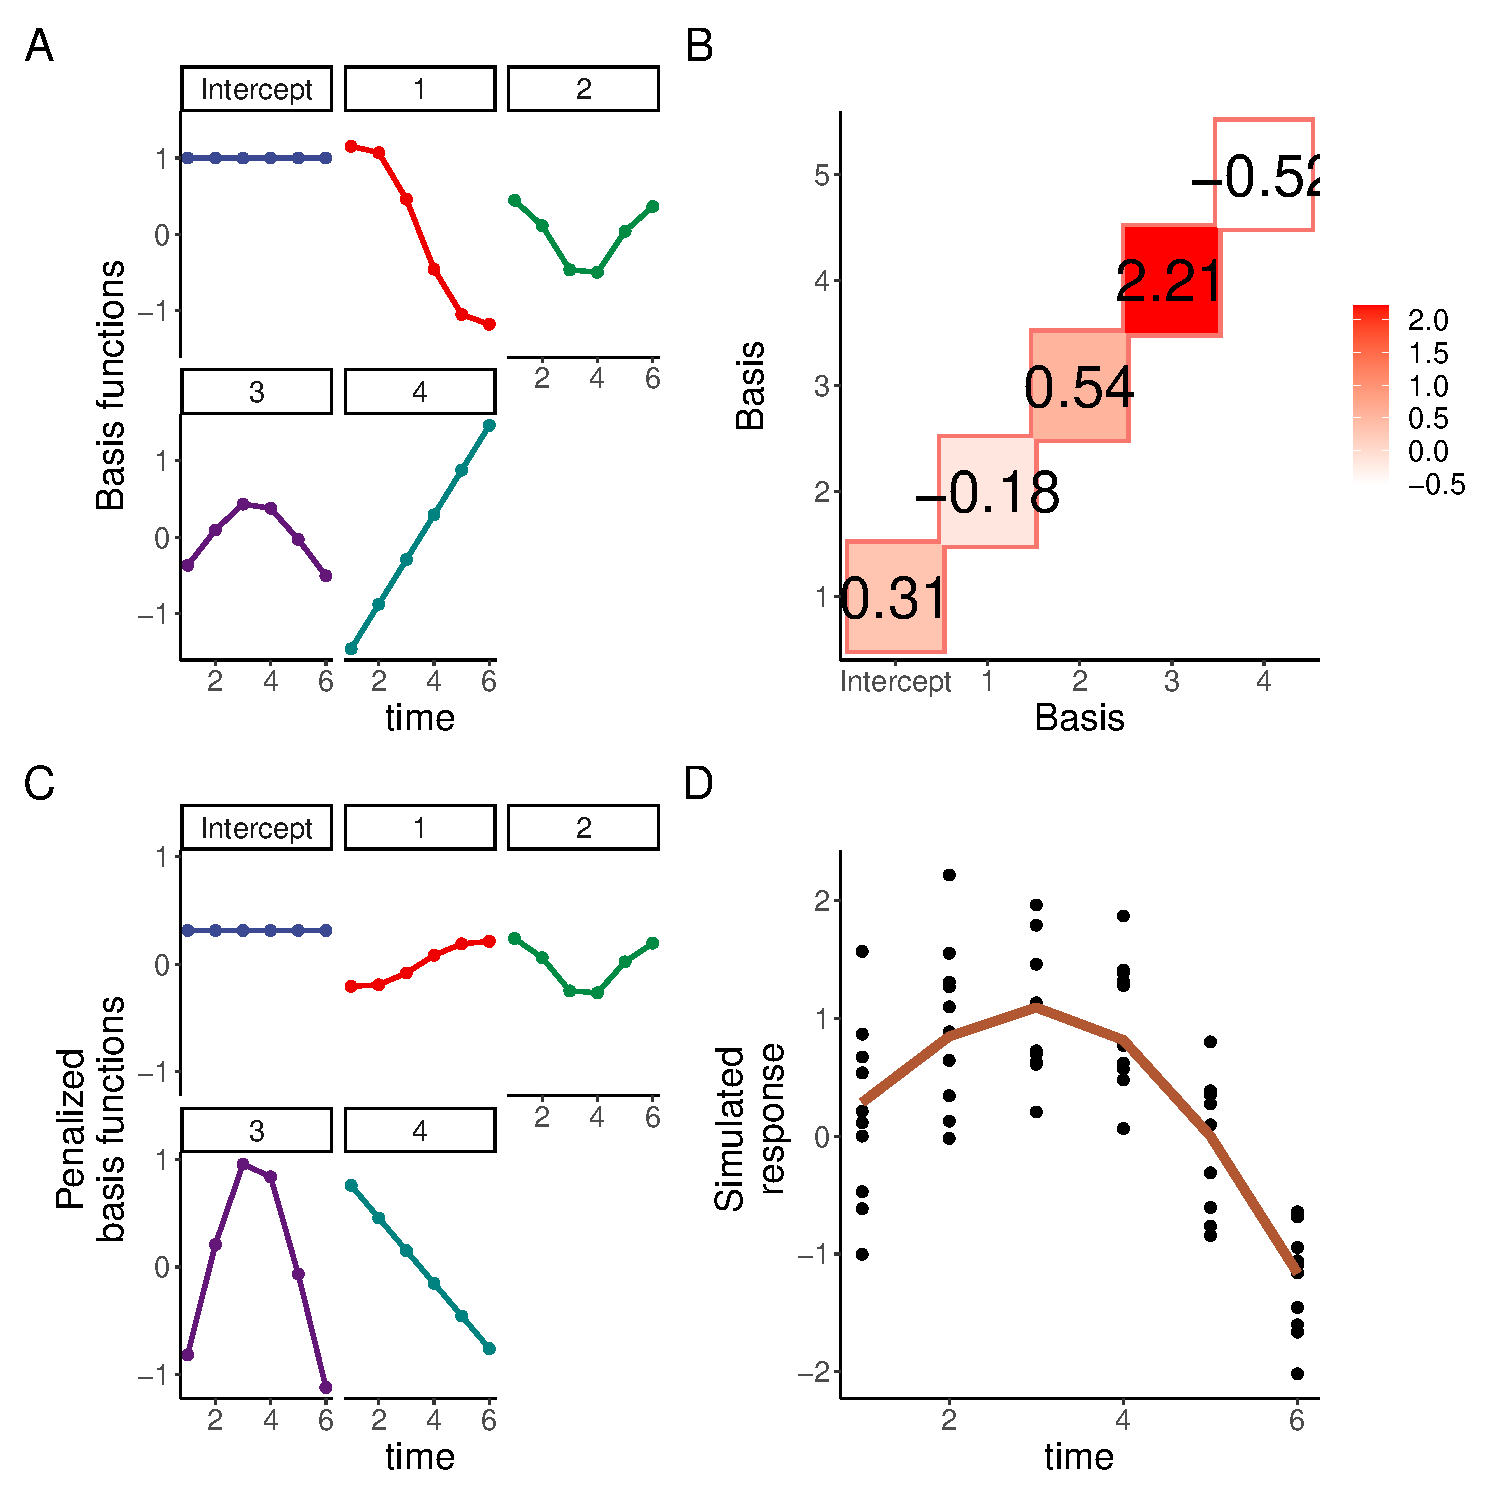
\includegraphics[width=0.75\linewidth,]{Manuscript_AM_v4_files/figure-latex/basis-plot-1} 

}

\caption{Basis functions for a single smoother for time with five knots. A: Basis functions for a single smoother for time for the simulated data of Group 1 from Figure 2, the intercept basis is not shown. B: Penalty matrix for the basis functions. Each basis function is penalized by a coefficient which can be positive or negative. The coefficient determines the overall effect of each basis in the final smoother. C: Penalized basis functions. Each of the four basis functions of panel A has been penalized by the corresponding coefficient shown in Panel B, note the corresponding increase (or decrease) of each basis. D. Smoother for time and original datapoints. The smoother (line) is the result of the sum of each penalized basis function at each time point, simulated values for the group appear as points.}\label{fig:basis-plot}
\end{figure}

\hypertarget{gams-and-covariance}{%
\subsection{GAMs and covariance}\label{gams-and-covariance}}

Although the specific methods of how GAMs model correlation structures is a topic beyond the scope of this work, it suffices to say that GAMs can handle correlation structures beyond compound symmetry. A detailed description on basis functions and correlations can be found in {[}52{]}. In a practical sense, when a GAM is implemented for longitudinal data, a spline can be added to the model for the \emph{time} effect to account for the repeated measures over time. An example where this is covered is in the Appendix.

\hypertarget{determination-of-significance-in-gams}{%
\subsection{Determination of significance in GAMs}\label{determination-of-significance-in-gams}}

At the core of a biomedical longitudinal study lies the question of a significant difference between the effect of two or more treatments in different groups. Whereas in rm-ANOVA a \emph{post-hoc} analysis is required to answer such question by calculating some \emph{p-values} after multiple comparisons, GAMs use a different approach to estimate significance. In essence, the idea behind the estimation of significance in GAMs across different treatment groups is that if the \emph{difference} between the confidence intervals of the fitted smooths for such groups is non-zero, then a significant difference exists at that timepoint (or timepoints). The absence of a \emph{p-value} in this case might seem odd, but when a confidence interval comparison is put into context the validity of its rationale becomes apparent. The major advantage of the significance estimation in GAMs is that they allow to determine significance at a specific timepoint, rather than providing a single \emph{p-value} for the overall treatment effect. The estimation of siginificant differences in GAMs is covered in detail in the Appendix using simulated longitudinal data that follows previously reported trends of tumor response between multiple treatment groups {[}16{]}.

\begin{center}\rule{0.5\linewidth}{0.5pt}\end{center}

\hypertarget{references}{%
\section*{References}\label{references}}
\addcontentsline{toc}{section}{References}

\hypertarget{refs}{}
\leavevmode\hypertarget{ref-roblyer2011}{}%
{[}1{]} D. Roblyer, S. Ueda, A. Cerussi, W. Tanamai, A. Durkin, R. Mehta, D. Hsiang, J.A. Butler, C. McLaren, W.-P. Chen, others, Optical imaging of breast cancer oxyhemoglobin flare correlates with neoadjuvant chemotherapy response one day after starting treatment, Proceedings of the National Academy of Sciences. 108 (2011) 14626--14631.

\leavevmode\hypertarget{ref-tank2020}{}%
{[}2{]} A. Tank, H.M. Peterson, V. Pera, S. Tabassum, A. Leproux, T. O'Sullivan, E. Jones, H. Cabral, N. Ko, R.S. Mehta, others, Diffuse optical spectroscopic imaging reveals distinct early breast tumor hemodynamic responses to metronomic and maximum tolerated dose regimens, Breast Cancer Research. 22 (2020) 1--10.

\leavevmode\hypertarget{ref-pavlov2018}{}%
{[}3{]} M.V. Pavlov, T.I. Kalganova, Y.S. Lyubimtseva, V.I. Plekhanov, G.Y. Golubyatnikov, O.Y. Ilyinskaya, A.G. Orlova, P.V. Subochev, D.V. Safonov, N.M. Shakhova, others, Multimodal approach in assessment of the response of breast cancer to neoadjuvant chemotherapy, Journal of Biomedical Optics. 23 (2018) 091410.

\leavevmode\hypertarget{ref-demidov2018}{}%
{[}4{]} V. Demidov, A. Maeda, M. Sugita, V. Madge, S. Sadanand, C. Flueraru, I.A. Vitkin, Preclinical longitudinal imaging of tumor microvascular radiobiological response with functional optical coherence tomography, Scientific Reports. 8 (2018) 1--12.

\leavevmode\hypertarget{ref-ritter2001}{}%
{[}5{]} G. Ritter, L.S. Cohen, C. Williams, E.C. Richards, L.J. Old, S. Welt, Serological analysis of human anti-human antibody responses in colon cancer patients treated with repeated doses of humanized monoclonal antibody a33, Cancer Research. 61 (2001) 6851--6859.

\leavevmode\hypertarget{ref-roth2017}{}%
{[}6{]} E.M. Roth, A.C. Goldberg, A.L. Catapano, A. Torri, G.D. Yancopoulos, N. Stahl, A. Brunet, G. Lecorps, H.M. Colhoun, Antidrug antibodies in patients treated with alirocumab, (2017).

\leavevmode\hypertarget{ref-jones2018}{}%
{[}7{]} J.D. Jones, H.E. Ramser, A.E. Woessner, K.P. Quinn, In vivo multiphoton microscopy detects longitudinal metabolic changes associated with delayed skin wound healing, Communications Biology. 1 (2018) 1--8.

\leavevmode\hypertarget{ref-skala2010}{}%
{[}8{]} M.C. Skala, A.N. Fontanella, L. Lan, J.A. Izatt, M.W. Dewhirst, Longitudinal optical imaging of tumor metabolism and hemodynamics, Journal of Biomedical Optics. 15 (2010) 011112.

\leavevmode\hypertarget{ref-greening2018}{}%
{[}9{]} G.J. Greening, K.P. Miller, C.R. Spainhour, M.D. Cato, T.J. Muldoon, Effects of isoflurane anesthesia on physiological parameters in murine subcutaneous tumor allografts measured via diffuse reflectance spectroscopy, Biomedical Optics Express. 9 (2018) 2871--2886.

\leavevmode\hypertarget{ref-sio2016}{}%
{[}10{]} T.T. Sio, P.J. Atherton, B.J. Birckhead, D.J. Schwartz, J.A. Sloan, D.K. Seisler, J.A. Martenson, C.L. Loprinzi, P.C. Griffin, R.F. Morton, others, Repeated measures analyses of dermatitis symptom evolution in breast cancer patients receiving radiotherapy in a phase 3 randomized trial of mometasone furoate vs placebo (N06C4 {[}alliance{]}), Supportive Care in Cancer. 24 (2016) 3847--3855.

\leavevmode\hypertarget{ref-kamstra2015}{}%
{[}11{]} J. Kamstra, P. Dijkstra, M. Van Leeuwen, J. Roodenburg, J. Langendijk, Mouth opening in patients irradiated for head and neck cancer: A prospective repeated measures study, Oral Oncology. 51 (2015) 548--555.

\leavevmode\hypertarget{ref-wagenmakers2008}{}%
{[}12{]} E.-J. Wagenmakers, M. Lee, T. Lodewyckx, G.J. Iverson, Bayesian versus frequentist inference, in: Bayesian Evaluation of Informative Hypotheses, Springer, 2008: pp. 181--207.

\leavevmode\hypertarget{ref-gueorguieva2004}{}%
{[}13{]} R. Gueorguieva, J.H. Krystal, Move over anova: Progress in analyzing repeated-measures data andits reflection in papers published in the archives of general psychiatry, Archives of General Psychiatry. 61 (2004) 310--317.

\leavevmode\hypertarget{ref-schober2018}{}%
{[}14{]} P. Schober, T.R. Vetter, Repeated measures designs and analysis of longitudinal data: If at first you do not succeed---try, try again, Anesthesia and Analgesia. 127 (2018) 569.

\leavevmode\hypertarget{ref-pinheiro2006}{}%
{[}15{]} J. Pinheiro, D. Bates, Mixed-effects models in s and s-plus, Springer Science \& Business Media, 2006.

\leavevmode\hypertarget{ref-vishwanath2009}{}%
{[}16{]} K. Vishwanath, H. Yuan, W.T. Barry, M.W. Dewhirst, N. Ramanujam, Using optical spectroscopy to longitudinally monitor physiological changes within solid tumors, Neoplasia. 11 (2009) 889--900.

\leavevmode\hypertarget{ref-dennis2019}{}%
{[}17{]} B. Dennis, J.M. Ponciano, M.L. Taper, S.R. Lele, Errors in statistical inference under model misspecification: Evidence, hypothesis testing, and aic, Frontiers in Ecology and Evolution. 7 (2019) 372.

\leavevmode\hypertarget{ref-wang2019}{}%
{[}18{]} B. Wang, Z. Zhou, H. Wang, X.M. Tu, C. Feng, The p-value and model specification in statistics, General Psychiatry. 32 (2019).

\leavevmode\hypertarget{ref-liu2010}{}%
{[}19{]} C. Liu, T.P. Cripe, M.-O. Kim, Statistical issues in longitudinal data analysis for treatment efficacy studies in the biomedical sciences, Molecular Therapy. 18 (2010) 1724--1730.

\leavevmode\hypertarget{ref-halsey2015}{}%
{[}20{]} L.G. Halsey, D. Curran-Everett, S.L. Vowler, G.B. Drummond, The fickle p value generates irreproducible results, Nature Methods. 12 (2015) 179--185.

\leavevmode\hypertarget{ref-abdi2010}{}%
{[}21{]} H. Abdi, Holm's sequential bonferroni procedure, Encyclopedia of Research Design. 1 (2010) 1--8.

\leavevmode\hypertarget{ref-nakagawa2004}{}%
{[}22{]} S. Nakagawa, A farewell to bonferroni: The problems of low statistical power and publication bias, Behavioral Ecology. 15 (2004) 1044--1045.

\leavevmode\hypertarget{ref-gelman2012}{}%
{[}23{]} A. Gelman, J. Hill, M. Yajima, Why we (usually) don't have to worry about multiple comparisons, Journal of Research on Educational Effectiveness. 5 (2012) 189--211.

\leavevmode\hypertarget{ref-albers2019}{}%
{[}24{]} C. Albers, The problem with unadjusted multiple and sequential statistical testing, Nature Communications. 10 (2019) 1--4.

\leavevmode\hypertarget{ref-ugrinowitsch2004}{}%
{[}25{]} C. Ugrinowitsch, G.W. Fellingham, M.D. Ricard, Limitations of ordinary least squares models in analyzing repeated measures data, Medicine and Science in Sports and Exercise. 36 (2004) 2144--2148.

\leavevmode\hypertarget{ref-huynh1976}{}%
{[}26{]} H. Huynh, L.S. Feldt, Estimation of the box correction for degrees of freedom from sample data in randomized block and split-plot designs, Journal of Educational Statistics. 1 (1976) 69--82.

\leavevmode\hypertarget{ref-greenhouse1959}{}%
{[}27{]} S.W. Greenhouse, S. Geisser, On methods in the analysis of profile data, Psychometrika. 24 (1959) 95--112.

\leavevmode\hypertarget{ref-haverkamp2017}{}%
{[}28{]} N. Haverkamp, A. Beauducel, Violation of the sphericity assumption and its effect on type-i error rates in repeated measures anova and multi-level linear models (mlm), Frontiers in Psychology. 8 (2017) 1841.

\leavevmode\hypertarget{ref-keselman2001}{}%
{[}29{]} H. Keselman, J. Algina, R.K. Kowalchuk, The analysis of repeated measures designs: A review, British Journal of Mathematical and Statistical Psychology. 54 (2001) 1--20.

\leavevmode\hypertarget{ref-charan2013}{}%
{[}30{]} J. Charan, N. Kantharia, How to calculate sample size in animal studies?, Journal of Pharmacology \& Pharmacotherapeutics. 4 (2013) 303.

\leavevmode\hypertarget{ref-barr2013}{}%
{[}31{]} D.J. Barr, R. Levy, C. Scheepers, H.J. Tily, Random effects structure for confirmatory hypothesis testing: Keep it maximal, Journal of Memory and Language. 68 (2013) 255--278.

\leavevmode\hypertarget{ref-rose2012}{}%
{[}32{]} N.L. Rose, H. Yang, S.D. Turner, G.L. Simpson, An assessment of the mechanisms for the transfer of lead and mercury from atmospherically contaminated organic soils to lake sediments with particular reference to Scotland, UK, Geochimica et Cosmochimica Acta. 82 (2012) 113--135.

\leavevmode\hypertarget{ref-pedersen2019}{}%
{[}33{]} E.J. Pedersen, D.L. Miller, G.L. Simpson, N. Ross, Hierarchical generalized additive models in ecology: An introduction with mgcv, PeerJ. 7 (2019) e6876.

\leavevmode\hypertarget{ref-simpson2018}{}%
{[}34{]} G.L. Simpson, Modelling palaeoecological time series using generalised additive models, Frontiers in Ecology and Evolution. 6 (2018) 149.

\leavevmode\hypertarget{ref-yang2012}{}%
{[}35{]} L. Yang, G. Qin, N. Zhao, C. Wang, G. Song, Using a generalized additive model with autoregressive terms to study the effects of daily temperature on mortality, BMC Medical Research Methodology. 12 (2012) 165.

\leavevmode\hypertarget{ref-beck1998}{}%
{[}36{]} N. Beck, S. Jackman, Beyond linearity by default: Generalized additive models, American Journal of Political Science. (1998) 596--627.

\leavevmode\hypertarget{ref-wood2017}{}%
{[}37{]} S.N. Wood, Generalized additive models: An introduction with r, CRC press, 2017.

\leavevmode\hypertarget{ref-r}{}%
{[}38{]} R Core Team, R: A language and environment for statistical computing, R Foundation for Statistical Computing, Vienna, Austria, 2020. \url{https://www.R-project.org/}.

\leavevmode\hypertarget{ref-wood2016}{}%
{[}39{]} S. Wood, N., Pya, B. Säfken, Smoothing parameter and model selection for general smooth models (with discussion), Journal of the American Statistical Association. 111 (2016) 1548--1575.

\leavevmode\hypertarget{ref-west2014}{}%
{[}40{]} B.T. West, K.B. Welch, A.T. Galecki, Linear mixed models: A practical guide using statistical software, CRC Press, 2014.

\leavevmode\hypertarget{ref-wolfinger1996}{}%
{[}41{]} R.D. Wolfinger, Heterogeneous variance: Covariance structures for repeated measures, Journal of Agricultural, Biological, and Environmental Statistics. (1996) 205--230.

\leavevmode\hypertarget{ref-weiss2005}{}%
{[}42{]} R.E. Weiss, Modeling longitudinal data, Springer Science \& Business Media, 2005.

\leavevmode\hypertarget{ref-geisser1958}{}%
{[}43{]} S. Geisser, S.W. Greenhouse, others, An extension of box's results on the use of the \(F\) distribution in multivariate analysis, The Annals of Mathematical Statistics. 29 (1958) 885--891.

\leavevmode\hypertarget{ref-maxwell2017}{}%
{[}44{]} S.E. Maxwell, H.D. Delaney, K. Kelley, Designing experiments and analyzing data: A model comparison perspective, Routledge, 2017.

\leavevmode\hypertarget{ref-molenberghs2004}{}%
{[}45{]} G. Molenberghs, H. Thijs, I. Jansen, C. Beunckens, M.G. Kenward, C. Mallinckrodt, R.J. Carroll, Analyzing incomplete longitudinal clinical trial data, Biostatistics. 5 (2004) 445--464.

\leavevmode\hypertarget{ref-scheffer2002}{}%
{[}46{]} J. Scheffer, Dealing with missing data, (2002).

\leavevmode\hypertarget{ref-potthoff2006}{}%
{[}47{]} R.F. Potthoff, G.E. Tudor, K.S. Pieper, V. Hasselblad, Can one assess whether missing data are missing at random in medical studies?, Statistical Methods in Medical Research. 15 (2006) 213--234.

\leavevmode\hypertarget{ref-ma2012}{}%
{[}48{]} Y. Ma, M. Mazumdar, S.G. Memtsoudis, Beyond repeated-measures analysis of variance: Advanced statistical methods for the analysis of longitudinal data in anesthesia research, Regional Anesthesia \& Pain Medicine. 37 (2012) 99--105.

\leavevmode\hypertarget{ref-nlme}{}%
{[}49{]} J. Pinheiro, D. Bates, S. DebRoy, D. Sarkar, R Core Team, nlme: Linear and nonlinear mixed effects models, 2020. \url{https://CRAN.R-project.org/package=nlme}.

\leavevmode\hypertarget{ref-nelder1972}{}%
{[}50{]} J.A. Nelder, R.W. Wedderburn, Generalized linear models, Journal of the Royal Statistical Society: Series A (General). 135 (1972) 370--384.

\leavevmode\hypertarget{ref-hastie1987}{}%
{[}51{]} T. Hastie, R. Tibshirani, Generalized additive models: Some applications, Journal of the American Statistical Association. 82 (1987) 371--386.

\leavevmode\hypertarget{ref-hefley2017}{}%
{[}52{]} T.J. Hefley, K.M. Broms, B.M. Brost, F.E. Buderman, S.L. Kay, H.R. Scharf, J.R. Tipton, P.J. Williams, M.B. Hooten, The basis function approach for modeling autocorrelation in ecological data, Ecology. 98 (2017) 632--646.

\leavevmode\hypertarget{ref-wegman1983}{}%
{[}53{]} E.J. Wegman, I.W. Wright, Splines in statistics, Journal of the American Statistical Association. 78 (1983) 351--365.

\end{document}
